% peer_poll.tex
\chapter{Peer/Poll Processes}
\label{cha:peer/poll_processes}

\section{Definitions}%
\label{sec:peer/poll_concepts}
Before discussing peer/poll processes in this chapter, we need to go through
some definitions. Some of them may not be clear at this point, we will discuss
them with more detail later.
\begin{enumerate}
    \item Offset $\theta$\\
        The maximum-likelihood time offset of the server clock relative to the
        system clock. It describes how different the client's time
        and the server's time are.
        % $$\theta_{AB} = \frac{1}{2}\left[\left(T_{i-2} - T_{i-3}\right) +
        % \left(T_{i-1} - T_i\right)\right]$$
    \item Delay $\delta$\\
        The round-trip delay between the client and server. It is equal to the
        amount of time that a message takes to travel from the client to the
        server plus the time for the return trip.
        % $$\delta_{AB} = \left(T_{i} - T_{i-3}\right) - \left(T_{i-1} -
        % T_{i-2}\right)$$
    \item Dispersion $\varepsilon$\\
        The maximum error inherent in the measurement of timestamps.
        Another definition: Potential clock offset error due to the maximum
        uncorrected system clock frequency error.  These definitions are in
        some respect confused, we will discuss them in greater detail in
        Section~\ref{sec:peer_processes}.
        % from website https://www.eecis.udel.edu/~mills/ntp/html/stats.html
    \item Jitter $\varphi$\\
        The root-mean-square (RMS) of a series of time offsets; this is used to
        indicate how stable the offset is.
\end{enumerate}

\section{Overview}%
\label{sec:peer_poll_overview}
The NTP ``on-wire protocol'' is used to send NTP packets between clients and
servers.  Figure~\ref{fig:peer_poll_processes} shows the basic architecture of
one peer/poll process. The communication between the client and one server
uses the NTP on-wire protocol (explained in the next section), which can
provide sample statistics ($\theta_0$, $\delta_0$, $t_0$ in the figure).  The most
recent eight samples are stored in a shift register, along with one more sample
statistic ($\varepsilon_i$). Then the peer process applies the clock
filter algorithm, which generates peer statistics ($\theta$, $\delta$,
$\varepsilon$, $\varphi$ in the figure), and passes them to the system process.


% figures/peer_poll_figure.tex

\begin{figure}[htpb]
\begin{center}
\begin{tikzpicture}[scale=0.7, transform shape,
        squarednode/.style={rectangle, draw=black, very thick, minimum
        size=10mm, minimum width=20mm, align=center},
        border/.style={draw=black, dashed, very thick},
    ]
    % Nodes
    % server
    \node[squarednode]  (s)                {Server};

    % on-wire protocol
    \node[align=center] (onwire) at ($(s.east) + (2.5, 2)$) {On-wire Protocol};
    \draw[border] ($(onwire.north west) + (-0.2, 0.2)$) -|
            ($(onwire.north east) + (0.2, -5)$) -|
            ($(onwire.north west) + (-0.2, 0.2)$);
    % poll process
    \node[squarednode] (poll) at ($(onwire) + (0, -6)$) {Poll Process};
    \draw[-latex, thick] (poll) |- ($(s.south) + (0, -0.5)$) -- (s);

    % shift registers
    \node[squarednode] (sr) at ($(onwire) + (4.5,-2)$) 
            {Shift Registers\\
            $(\theta_1, \delta_1, \varepsilon_1, t_1)$\\
            $(\theta_2, \delta_2, \varepsilon_2, t_2)$\\
            $(\theta_3, \delta_3, \varepsilon_3, t_3)$\\
            $(\theta_4, \delta_4, \varepsilon_4, t_4)$\\
            $(\theta_5, \delta_5, \varepsilon_5, t_5)$\\
            $(\theta_6, \delta_6, \varepsilon_6, t_6)$\\
            $(\theta_7, \delta_7, \varepsilon_7, t_7)$\\
            $(\theta_8, \delta_8, \varepsilon_8, t_8)$
            };
    \draw[-latex, thick] (s) -- (sr) node[midway, above] 
            {$(\theta_0, \delta_0, t_0)$};
    % clock filter algorithm
    \node[squarednode] (cf) [right=of sr] {Clock Filter\\ algorithm};
    \draw[-latex, thick] (sr) -- (cf);

    % peer process
    \node[align=center] (peer) [below=2mm of sr.south east] {Peer Process};
    \draw[border] ($(sr.north west) + (-0.5, 0.2)$) -- 
            ($(sr.south west) + (-0.5, -1.2)$)
            -|
            ($(cf.east) + (0.2, 0)$) |-
            ($(sr.north west) + (-0.5, 0.2)$);


    % system process
    \node[squarednode] (sp) [right=2.5 of cf] {System process};
    \draw[-latex, thick] (cf) -- (sp) node[midway, above] 
            {$(\theta, \delta, \varepsilon, \varphi)$};
    
    % synchronizations
    % \draw[-latex, ultra thick] (s1) -- (rc);

\end{tikzpicture}
\end{center}
\caption{Peer/Poll processes}
\label{fig:peer_poll_processes}
\end{figure}



% fig:peer_poll_processes

The purpose of the peer processes is to communicate with servers and to
calculate and keep statistics of the communications which can be used to
determine how reliable the time estimates received from the servers are. Poll
processes are used to manage the communications to get sufficient data without
making the servers too busy.

\section{On-wire protocol}%
\label{sec:on_wire_protocol}
In an NTP subnet, a client can send a request to a server and the server sends
back a response. This whole round of communication can generate one sample. For
every sample, the client wants to know the difference between the server's
system clock and its own clock (i.e., the offset).  However, it may take a
while for the server to generate and send the response. This delay is not
predictable, as well as the network delay between the two devices. In an NTP
subnet, clients and servers communicate using an on-wire protocol. It provides
a smart way to calculate the offset and delay for every sample. 

\subsection{Statistics calculation}%
\label{sub:statistics_calculation}
Figure~\ref{fig:on_wire1} represents the timestamps and communications between
a client and a server. The vertical dashed line indicates the same time. The
arrow indicates the communication packets sent from one side and received at
the other side. The notation $T_i$ stands for the timestamp obtained from the
system clock of one device. Note that these timestamps are times of a given
computer system's clock, which is (in general) only an approximation to the
actual time.

% figures/on_wire1.tex

\begin{figure}[htpb]
\begin{center}
\begin{tikzpicture}[scale=0.7, transform shape,
        textnode/.style={rectangle, very thick, minimum
        size=10mm, minimum width=20mm, align=center},
        border/.style={draw=black, dashed, very thick},
        arrow/.style={-latex, ultra thick},
    ]
    % server
    \node[textnode]  (s)                {Server};
    \draw[arrow]     (s) -- ($(s) + (10,0)$);

    % client
    \node[textnode]  (c)    [below=20mm of s]            {Client};
    \draw[arrow]     (c) -- ($(c) + (10,0)$);

    % communications
    \draw[arrow]     ($(c) + (5, 0)$) -- ($(s) + (6, 0)$);
    \draw[arrow]     ($(s) + (8, 0)$) -- ($(c) + (9, 0)$);

    % vertical line
    \draw[border]    ($(s) + (3, 1)$) -- ($(c) + (3, -1)$);

    % labels
    \node[textnode] at ($(c) + (2.5, -0.5)$)   {$t_0$};
    \node[textnode] at ($(s) + (2.5, 0.5)$)    {$t_1$};
    \node[textnode] at ($(c) + (5, -0.5)$)   {$t_2$};
    \node[textnode] at ($(s) + (6, 0.5)$)    {$t_3$};
    \node[textnode] at ($(s) + (8, 0.5)$)    {$t_4$};
    \node[textnode] at ($(c) + (9, -0.5)$)   {$t_5$};

\end{tikzpicture}
\end{center}
\caption{Time stamps}
\label{fig:on_wire1}
\end{figure}



% fig:on_wire1

In an ideal situation, if we have $T_1$ and $T_0$, which are timestamps
obtained from both devices at the same instant, then we can get the offset
$\theta$:
$$\theta = T_1 - T_0$$
However, we cannot do this since we cannot determine whether two timestamps
were taken at the same time. The NTP on-wire protocol calculates the
offset in an alternative way:
\begin{equation}
    \theta = \frac{1}{2}\left[(T_3 - T_2) + (T_4 - T_5)\right]
    \label{eq:offset_def}
\end{equation}
Note that this equation is equivalent to:
$$\theta = \frac{T_3 + T_4}{2} - \frac{T_2 + T_5}{2}$$
which means that the offset is equal to the difference between two timestamps
which are the middle points of $[T_3, T_4]$ and $[T_2, T_5]$. 
If the network delay is symmetric, which means the time for packets to travel
from client to server and the time for packets to get back are equal, the
middle points are at the same time. In this case, it is equivalent to the ideal
situation. If the delay is asymmetric, there will be an error of the
calculation in that the calculated offset is biased by the degree of asymmetry
of the delays. It is not possible to correct this error. However, there is one
scenario in which the error can be attenuated~\cite{redbook}. We will discuss this
part in Section~\ref{sub:huff_n_puff_filter}.

The delay $\delta$ is calculated by:
\begin{equation}
    \delta = (T_5 - T_2) - (T_4 - T_3)
    \label{eq:delay_def}
\end{equation}
This delay is actually a difference of two time periods. It is not impacted by
the offset, since each time period is calculated using two timestamps from the
same device. 

As mentioned in Section~\ref{sec:adjusting_system_time}, the frequency of 
the system clock may not be accurate. This inaccuracy also impacts the
calculations here. We will discuss this more in
Section~\ref{sec:phase_frequency_prediction} and
Section~\ref{sec:intrinsic_frequency_offset}.

There is another statistic $t$ in Figure~\ref{fig:peer_poll_processes}, which
indicates the time at which the offset $\theta$ and delay $\delta$ are
calculated.  In practice we can let $t = T_5$, because it is just used to
indicate the order of groups of sample statistics, we do not need it to be
extremely accurate.  In Figure~\ref{fig:peer_poll_processes}, we add the
subscript 0 to distinguish the newest group of sample statistics from the
groups which are in the shift register.

\subsection{Timestamps in NTP packet}%
\label{sub:timestamps_in_ntp_packet}
% how to store timestamps and modes
% https://www.eecis.udel.edu/~mills/onwire.html
NTP uses NTP packets in communications. The NTP packet is a UDP
datagram~\cite{rfc5905}. There are four timestamps in the NTP packet header:
\begin{enumerate}
    \item Reference Timestamp\\
        The time when the system clock was last set or corrected. When this
        timestamp is in the header of an NTP packet from a server, this
        timestamp means when the server's system clock was last set or
        corrected. Note that this timestamp is useless in the header of an NTP
        packet which is sent from a client to a server. 
    \item Origin Timestamp (\emph{org})\\
        The time at the client when the request packet departs.
    \item Receive Timestamp (\emph{rec})\\
        The time at the server when the request packet was received.
    \item Transmit Timestamp (\emph{xmt})\\
        The time at the server when the response packet departs.
\end{enumerate}
In the peer process, we are interested in another time: destination
timestamp (\emph{dst}), which is the time at the client when it receives the
response packet. The reference timestamp is not used in the calculation below.
All timestamps are 64-bit numbers. The first 32 bits represent the
number of seconds since 00:00 January 1 1900 UTC~\cite{rfc5905}. The second 32
bits are used as the fractional part, which provides a resolution of 232
picosecondes. Referring to Figure~\ref{fig:on_wire1}, the packet which leaves
at $T_4$ contains $T_4$, $T_3$ and $T_2$ in its header, where $$ \textit{org} =
T_2,~\textit{rec} = T_3,~\text{and }\textit{xmt} = T_4 $$ When the client gets
the packet, it captures $\textit{dst} = T_5$.

The purpose of the on-wire protocol is to calculate the offset $\theta$ and
delay $\delta$ based on the communication. The four timestamps used in
Equation~\ref{eq:offset_def} and Equation~\ref{eq:delay_def} are important,
they are \emph{org}, \emph{rec}, \emph{xmt} and \emph{dst}.  High accuracy
requires that they are captured as close to the actual time of the relative
event (sending or receiving a packet) as possible. The on-wire protocol
provides two interleaved modes which are known as \emph{interleaved symmetric}
and \emph{interleaved broadcast}. They are extensions of the basic symmetric
mode and basic broadcast mode, respectively~\cite{on_wire}.
%
In the basic modes, \emph{org} and \emph{xmt} in the outgoing packet are
captured before the packet is made, which is not the timestamp when the packet
is actually sent. 
This kind of timestamp is called a \emph{softstamp}. In this case, 
after a softstamp is captured, there are additional operations to do before
sending the packet, such as adding validation information to the packet and
adding the packet to the output queue; then the packet will wait in the queue
before it is sent.  For \emph{rec} and \emph{dst}, which are also called
\emph{drivestamps}, they are captured ``shortly after the input device
interrupt and before adding the buffer to the input queue''\cite{on_wire}. We
can see that the drivestamps are more accurate than the softstamps because
there is only a short delay in handling the interrupt. If we can capture
timestamps exactly when packets are sent or received, they will be more
accurate. However, we need additional hardware support to do this.

In interleaved modes, we can make softstamps more accurate without
additional hardware support. The trade off is that we need more packets.
Instead of capturing softstamps before the packets are made, we can capture
them shortly after the output interrupt. In this case, the accuracy is similar
to that of drivestamps but they can not be sent in the same packet as the one
whose transmission time they represent. We need one more packet if we want to
send this kind of softstamps. More detail about interleaved modes is beyond
the scope of this thesis.

\subsection{Non-reliable protocol}%
\label{sub:non_reliable_protocol}
As mentioned in Section~\ref{sub:timestamps_in_ntp_packet}, the NTP packet is a
UDP datagram. This makes the on-wire protocol not reliable, which means that
there is no guarantee about the delivery of packets. Possibly
counterintuitively, reliable delivery actually
decreases the reliability of NTP packets. Assume we are implementing the
on-wire protocol to make it reliable by using techniques similar to TCP, a lost
packet will be sent again. However, an identical packet is not valid since the
timestamp which indicates the time when the packet was sent is incorrect.

\subsection{Example}%
\label{sub:example}
Assume a client sent a request to one server and got a response. Suppose the four
timestamps are:
$$
\textit{org} = T_2 = 3762785257.12414
$$
$$
\textit{rec} = T_3 = 3762785257.13128 
$$
$$
\textit{xmt} = T_4 = 3762785257.15132
$$
$$
\textit{dst} = T_5 = 3762785257.16213 
$$
We can calculate the offset:
\begin{align*}
\theta & = \frac{1}{2}\left[(T_3 - T_2) + (T_4 - T_5)\right]\\
       & = \frac{1}{2}[(3762785257.13128 - 3762785257.12414) \\
       & \quad + (3762785257.15132 - 3762785257.16213)]\\
       & = -0.001835
\end{align*}
and the delay:
\begin{align*}
\delta & = (T_5 - T_2) - (T_4 - T_3) \\
       & = (3762785257.16213 - 3762785257.12414) \\
       & \quad - (3762785257.15132 - 3762785257.13128) \\
       & = 0.01795
\end{align*}
thus we have the offset is 1.835 ms and the delay is 17.95 ms.

\section{Peer processes}%
\label{sec:peer_processes}
As shown in Figure~\ref{fig:peer_poll_processes}, 
for each server, the on-wire protocol provides sample statistics $\theta$,
$\delta$ and $t$ and passes them to the peer process. Then the peer process
maintains them and the clock filter algorithm calculates peer statistics based
on them.

\subsection{Sample statistics maintenance}%
\label{sub:sample_statistics_maintenance}
As mentioned in Section~\ref{sec:peer_poll_overview}, there is a shift register
which stores the most recent eight samples. When a packet arrives, the peer
process replaces the oldest sample by the new one with an added dispersion
$\varepsilon$.
The dispersion is initialized as:
$$ \varepsilon = \rho_r + \rho_s + \phi (T_5 - T_2) $$
where 
\begin{itemize}
    \item 
        $\rho_r$ is the packet precision in the NTP packet header. 
        % It represents the system precision of the server.
    \item 
        $\rho_s$ is the system
        precision which we discuss below.
    \item
        $\phi = 15 ppm = 15 \mu s/s$ is a constant.
    \item
        $T_5$ and $T_2$ are the two timestamps shown in
        Figure~\ref{fig:on_wire1}. In other words, $T_5$ is \emph{dst} and
        $T_2$ is \emph{org}.
\end{itemize}
After storing the sample statistics into the shift register, the dispersion
is increased at a constant rate $\phi$. 

The system precision is automatically determined by NTP; it represents 
``the smallest possible increase of time that can be experienced by a
program''~\cite{precision}.

In Section~\ref{sec:peer/poll_concepts} we mentioned that dispersion is the
maximum error. Now we can consider dispersion as a function of time ($t$) and
we have:
\begin{equation}
    \varepsilon(t) = \rho_r + \rho_s + \phi (t - T_2)
    \label{eq:dispersion}
\end{equation}
In Equation~\ref{eq:dispersion}, dispersion has two parts. $\rho_r + \rho_s$
represents the error due to the precisions of the server and client clocks,
while $\phi (t - T_2)$ represents the error due to frequency tolerance and
time.  The $\phi = 15ppm$ is a frequency tolerance which represent the maximum
frequency offset after the intrinsic frequency offset is determined as
described in Section~\ref{sec:intrinsic_frequency_offset}.

\subsection{Initial and invalid samples}%
\label{sub:initial_and_invalid_samples}
When the NTP service starts, all eight groups of sample statistics in the shift
register are initialized to the dummy tuple: $\theta = 0$, $\delta =
\verb|MAXDISP|$, $\varepsilon = \verb|MAXDISP|$ and $t = 0$, where $\verb|MAXDISP|
= 16$ is the maximum dispersion~\cite{rfc5905}.

There is a 8-bit shift register called the ``reach register'' which is
shared by the peer
and poll process and used to determine whether the server is reachable and the
data is fresh. It is maintained by the poll process, which we will discuss in
Section~\ref{sec:poll_processes}. After a packet is sent to the server, the
register is shifted left by one bit and the rightmost bit is set to 0. If a
valid packet arrives from the server, the rightmost bit is set to 1. A
server is reachable only when there is at least one non-zero bit in the
register. If the three rightmost bits are all 0, there will be a dummy tuple of
sample statistics
inserted into the shift register by replacing the oldest one. The dummy sample
indicate an invalid sample. If the eight bits are all 0, we consider the
server as unreachable.

\subsection{Clock filter algorithm}%
\label{sub:clock_filter_algorithm}
The clock filter algorithm calculates peer statistics used in the system
process.  As mentioned in Section~\ref{sec:peer_poll_overview}, there are eight
groups of sample statistics in the shift register. The clock filter algorithm
selects one of them to represent the offset and delay of the server, then
calculates the peer dispersion and jitter, and then passes them, as well as the
arrival time of the selected sample, to the system process.

Figure~\ref{fig:clock_filter} is ``a wedge scattergram plotting sample points
of offset versus delay collected over a 24-hr period''~\cite{clock_filter}. It
shows that as the delay increases, the variance of offset increases as
well. In this case, the best sample should be the one with the lowest delay. We
will discuss this more in Section~\ref{sub:huff_n_puff_filter}.

% clock_filter

\begin{figure}[htb]
    \centering
    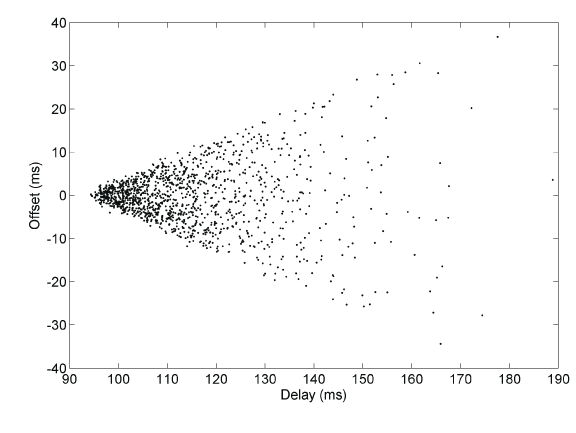
\includegraphics[width=0.5\textwidth]{figures/clock_filter.png}
    \caption{Wedge Scattergram}
    \label{fig:clock_filter}
\end{figure}


% fig:clock_filter

Based on the information seen in Figure~\ref{fig:clock_filter}, the clock filter
algorithm first sorts the samples by their delay. If the first sample is later
than the last sample we selected, it is selected; otherwise nothing more
happens. This mechanism guarantees that a sample will be used at most
once.

After the selection, the offset $\theta$ and delay $\delta$ of the sample
become peer statistics with the same names. The sorted samples are indexed from
0 to 7, from the one with the lowest delay to the one with highest. Here
$\varepsilon_i$ indicates the dispersion of the sample with index $i$. We
calculate peer dispersion $\varepsilon$ by:
\begin{equation}
    \varepsilon = \sum^{7}_{i=0} \frac{\varepsilon_i}{2^{(i+1)}}
    \label{eq:peer_dispersion}
\end{equation}
The peer jitter $\varphi$ is calculated by:
\begin{equation}
    \varphi = \sqrt{\frac{1}{n-1} \sum^{n-1}_{j=1} (\theta_0 - \theta_j)^2}
    \label{eq:peer_jitter}
\end{equation}
where $n$ is the number of valid samples in the shift register ($n > 1$).
The peer jitter is the root-mean-square (RMS) of differences between sample
offsets and the sample offset of the selected sample: ``it represents the
nominal error in estimating the offset''~\cite{rfc5905}. A larger jitter
indicates that the offset varies more; in that case, we can consider that there
may be some problem with the server and/or the connection, since the offset
should not change much if we did not adjust the client's system clock by a
large amount.

\subsection{Example}%
\label{sub:example}
Assume that for a given peer, we have eight samples in the shift register; the
offsets, delays and dispersions are as shown in Table~\ref{tab:clock_filter},
\begin{table}[htpb]
    \centering
    \caption{Eight samples in shift register}
    \label{tab:clock_filter}
    \begin{tabular}{|c|c|c|c|}
        \hline
        Index after sorting ($i$) & offset $\theta_i$ & delay $\delta_i$ 
        & dispersion $\varepsilon_i$ \\
        \hline
        4& -31.87&  165.34&  0.459\\
        \hline
        7&  -5.04&  193.85&  1.202\\
        \hline
        6& -42.67&  175.49&  2.303\\
        \hline
        3& -15.21&  156.37&  3.355\\
        \hline
        2& -10.36&  117.40&  4.161\\
        \hline
        1&  23.99&   73.12&  5.137\\
        \hline
        5&  -3.81&  166.99&  5.948\\
        \hline
        0&  34.04&   64.09&  6.842\\
        \hline
    \end{tabular}
\end{table}
where the units of offset, delay and dispersion are milliseconds.
Table~\ref{tab:clock_filter} shows the indices of of the samples after sorting
them by their delay. In this example, the peer offset will be 34.04 ms and the
peer delay will be 64.09~ms. The peer dispersion $\varepsilon$ is:
$$ \varepsilon = \sum^{7}_{i=0} \frac{\varepsilon_i}{2^{(i+1)}} = 11.13
\text{ ms} $$
and the peer jitter is 
$$
    \varphi = \sqrt{\frac{1}{n-1} \sum^{n-1}_{j=1} (\theta_0 - \theta_j)^2}
    = 52.27 \text{ ms}
$$

\subsection{Huff-n'-puff filter}%
\label{sub:huff_n_puff_filter}
Now we are going to look at Figure~\ref{fig:clock_filter} more closely. In the
figure, ``there are two limb lines at slope $\pm0.5$, representing the
limits of sample variation''~\cite{clock_filter}.
The variation of offset is caused by the asymmetric delay, and it is actually
an error.

Figure~\ref{fig:huff_n_puff1} shows the relationship between
delay and offset error.  Figure~\ref{subfig:best_case} shows the best case,
where the delays are symmetric. In this case, the middle points which are
indicated by the ends of the dashed line (the other two figures are the same)
are at the same time. As we mentioned in
Section~\ref{sub:statistics_calculation}, the calculation in
Equation~\ref{eq:offset_def} is correct. 

% figures/huff_n_puff1.tex

\begin{figure}[htpb]
\begin{center}
\subfloat[Best case]{
\begin{tikzpicture}[scale=0.73, transform shape,
        textnode/.style={rectangle, very thick, minimum
        size=10mm, minimum width=20mm, align=center},
        border/.style={draw=black, dashed, very thick},
        arrow/.style={-latex, ultra thick},
    ]
    % server
    \node[textnode]  (s)                        {Server};
    \draw[arrow]     (s) -- ($(s) + (9,0)$);

    % client
    \node[textnode]  (c)    [below=20mm of s]   {Client};
    \draw[arrow]     (c) -- ($(c) + (9,0)$);

    % communications
    \draw[arrow]     ($(c) + (3, 0)$) -- ($(s) + (3.5, 0)$);
    \draw[arrow]     ($(s) + (6.5, 0)$) -- ($(c) + (7, 0)$);

    % dash line
    \draw[border]    ($(s) + (5, 0)$) -- ($(c) + (5, 0)$);
\end{tikzpicture}
\label{subfig:best_case}
}
\subfloat[Normal case]{
\begin{tikzpicture}[scale=0.7, transform shape,
        textnode/.style={rectangle, very thick, minimum
        size=10mm, minimum width=20mm, align=center},
        border/.style={draw=black, dashed, very thick},
        arrow/.style={-latex, ultra thick},
    ]
    % server
    \node[textnode]  (s)                        {Server};
    \draw[arrow]     (s) -- ($(s) + (9.5,0)$);

    % client
    \node[textnode]  (c)    [below=20mm of s]   {Client};
    \draw[arrow]     (c) -- ($(c) + (9.5,0)$);

    % communications
    \draw[arrow]     ($(c) + (3, 0)$) -- ($(s) + (4, 0)$);
    \draw[arrow]     ($(s) + (6, 0)$) -- ($(c) + (7.5, 0)$);

    % dash line
    \draw[border]    ($(s) + (5, 0)$) -- ($(c) + (5.25, 0)$);
\end{tikzpicture}
\label{subfig:normal_case}
}

\subfloat[Extremely asymmetric case]{
\begin{tikzpicture}[scale=0.7, transform shape,
        textnode/.style={rectangle, very thick, minimum
        size=10mm, minimum width=20mm, align=center},
        border/.style={draw=black, dashed, very thick},
        arrow/.style={-latex, ultra thick},
    ]
    % server
    \node[textnode]  (s)                        {Server};
    \draw[arrow]     (s) -- ($(s) + (10,0)$);

    % client
    \node[textnode]  (c)    [below=20mm of s]   {Client};
    \draw[arrow]     (c) -- ($(c) + (10,0)$);

    % communications
    \draw[arrow]     ($(c) + (3, 0)$) -- ($(s) + (3, 0)$);
    \draw[arrow]     ($(s) + (5, 0)$) -- ($(c) + (7.5, 0)$);

    % dash line
    \draw[border]    ($(s) + (4, 0)$) -- ($(c) + (5.25, 0)$);
    \draw[border]    ($(s) + (4, 0)$) -- ($(c) + (4, 0)$);

    % labels
    \node[textnode] at ($(c) + (3, -0.5)$)      {$T_0$};
    \node[textnode] at ($(s) + (3, 0.5)$)       {$T_1$};
    \node[textnode] at ($(s) + (5, 0.5)$)       {$T_2$};
    \node[textnode] at ($(c) + (7.5, -0.5)$)    {$T_3$};
    \node[textnode] at ($(s) + (4, 0.5)$)       {$T_4$};
    \node[textnode] at ($(c) + (5.25, -0.5)$)   {$T_5$};
    \node[textnode] at ($(c) + (4, -0.5)$)      {$T_6$};

\end{tikzpicture}
\label{subfig:extremely_asymmetric_case}
}
\end{center}
\caption{The relationship between delay and offset variance}
\label{fig:huff_n_puff1}
\end{figure}



% fig:huff_n_puff1

Figure~\ref{subfig:normal_case} shows a typical case in which the delays are
slightly different; this makes the middle points slightly different as well.
This difference leads an error in the calculation of the offset.

Figure~\ref{subfig:extremely_asymmetric_case} represents an extremely
asymmetric case, where there is no upload delay and the download delay is
relatively large. If $T_6$ and $T_4$ are captured at the same time, then the
error of offset is the difference between $T_5$ and $T_6$. We can prove that it
is equal to $-\frac{1}{2}\delta$. In another case, if the upload delay is
relatively large and the download delay is zero, the error is equal to
$\frac{1}{2}\delta$. Note that these cases are the situations when the error is
maximum.

With this analysis, we know that the slope $\pm0.5$ is not determined by
experiment, but is calculated in theory and we know the variation of offset is
actually error, which is the reason that we select the sample with smallest
delay, which leads to smallest offset error.

The clock filter algorithm works best when there is a symmetric delay, as
Figure~\ref{fig:huff_n_puff1} shows. It is also mentioned that the errors due
to asymmetric delay are almost unable to be corrected~\cite{redbook}. However,
the huff-n'-puff filter is used to attenuate these errors.

Figure~\ref{fig:huff_n_puff2}~\cite{huff_n_puff} shows a scattergram like
Figure~\ref{fig:huff_n_puff1}, but the network delay is much more asymmetric.
From the figure, we find that the samples are close to the upper limb line,
which indicates that the offset error is positive. This means that the upload
delay is larger than the download delay. (Note that document~\cite{huff_n_puff}
shows the opposite opinion, which is an error in the
document.) By applying the huff-n'-puff filter, we can do the following:
\begin{itemize}
    \item 
        Remember the recent sample with lowest delay, where ``recent'' usually
        means ``recent hours''. The offset and delay of the sample are denoted
        by $\theta_0$ and $\delta_0$. Note that the sample is near the apex of
        the data in the scattergram.
    \item 
        For a new sample whose offset and delay are $\theta_i$ and
        $\delta_i$, we keep its delay value and adjust its offset as follows:
        \begin{equation}
            \theta = 
            \begin{cases}
                \displaystyle
                \theta_i - \frac{\delta_i - \delta_0}{2}, &\text{ if }\theta_i
                > \theta_0\\
                \displaystyle
                \theta_i + \frac{\delta_i - \delta_0}{2}, &\text{ if }\theta_i
                < \theta_0\\
            \end{cases}
            \label{eq:huff_n_puff}
        \end{equation}
\end{itemize}

% figures/huff_n_puff2.tex

\begin{figure}[htb]
    \centering
    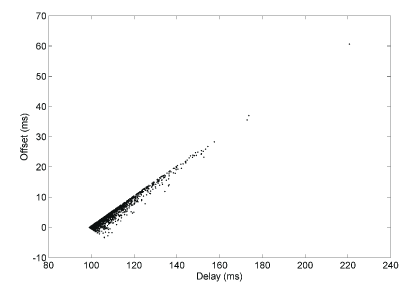
\includegraphics[width=0.8\textwidth]{figures/huff_n_puff.png}
    \caption{Huff-n'-puff Wedge Scattergram}
    \label{fig:huff_n_puff2}
\end{figure}


% fig:huff_n_puff2

Note that this adjustment is actually moving the sample points close to the
horizontal line which goes through the point $(\delta_0, \theta_0)$, if the
samples are near the upper limb line, as Figure~\ref{fig:huff_n_puff2} shows.
It is also said that it is less effective and will lead to significant errors
when a large amount of samples are in the area between the limb
lines~\cite{huff_n_puff}. If the actual situation is like
Figure~\ref{fig:huff_n_puff2}, the adjustment works fine, since it can avoid
the variation of offset which can be considered as error.

%\subsection{Reachability detection}%
%\label{sub:reachability_detection}
% https://docs.ntpsec.org/latest/stats.html
% redbook

\section{Poll processes}%
\label{sec:poll_processes}
As mentioned in Section~\ref{sec:peer_poll_overview}, poll processes are
designed to control the interval of communications in order to get sufficient
data without making servers too busy. 

The key part of the poll process is the time constant $T_c$ and its
exponent $\uptau$ where $T_c = 2 ^ {\uptau}$. A client sends poll requests to
each server with a \emph{poll interval} of $T_c$ seconds. The exponent $\uptau$
is a whole number and is called the \emph{poll exponent}, which ranges from 4
to 17~\cite{rfc5905}.  
$T_c$ and $\uptau$ are maintained by the clock discipline process. This is
discussed later in Chapter~\ref{cha:clock_discipline_process}.

There are two options to the poll process: \verb|BURST| and \verb|IBURST|\null.
With the \verb|BURST| option, instead of sending one request at each poll
interval, the poll process sends 8 packets. The interval between packets is two
seconds.  With the \verb|IBURST| option, when a server is unreachable, it sends
8 packets at two seconds intervals. The \verb|IBURST| option is used to reduce
the synchronization time at initial start up while the \verb|BURST| option can
reduce noise at long poll intervals~\cite{poll_process}.

In next chapter, we will have a look at how system process handle the
statistics calculated here.
